%! TeX root: ../informe.tex
\section{Introducción}

\section{2a Sección}
\label{sec:2Seccion}

\section{3a Sección}
\label{sec:3Seccion}

\textbf{Items:}

\begin{itemize}
	\item 1er Item.
  \item 2do Item.
  \item er Item.
\end{itemize}

\textbf{Enumeraciones:}

\begin{enumerate}
	\item 1.1 Elemento.
	\item 1.2 Elemento.
  \begin{enumerate}
		\item 2.1 Elemento.
		\item 2.2 Elemento.
  \end{enumerate}
	\item 1.3 Elemento.
\end{enumerate}

\section{4ª Sección}
\label{sec:4Sección}

\subsection{Sub Sección 4.1}
\label{sec:41SubSección}

\subsection{Sub Sección 4.2}
\label{sec:42SubSección}

\section{5ª Sección}
\label{sec:Sección4}

\subsection{Sub Sección 5.1}
\label{sec:51SubSección}

\subsubsection{Sub Sub Sección 5.1.1}
\label{sec:511SubSubSección}

\subsubsection{Sub Sub Sección 5.1.2}
\label{sec:512SubSubSección}

\subsubsection{Sub Sub Sección 5.1.3}
\label{sec:513SubSubSección}

\subsubsection{Sub Sub Sección 5.1.4}
\label{sec:514SubSubSección}

\subsubsection{Sub Sub Sección 5.1.5}
\label{sec:515SubSubSección}

\subsection{Sub Sección 5.2}
\label{sec:52SubSección}

%\begin{longtable}[htbp]
\begin{longtable}
%	\centering
%		\begin{tabular}{|p{7cm}|p{7cm}|} \hline
		{|p{7cm}|p{7cm}|} \hline
		  \textbf{1ª Columna} & \textbf{2ª Columna} \\ \hline 
			Celda 1.1 & Celda 1.2  \\ \hline
			Celda 2.1 & Celda 2.2\footnotemark[1] \textbf{Con Nota al Pie} \\ \hline 
			Celda 3.1 & Celda 3.2 \\ \hline 
			Celda 4.1 & Celda 4.2 \\ \hline
			Celda 5.1 & Celda 5.2 \\ \hline
			Celda 6.1 & Celda 6.2 \\ \hline 
			Celda 7.1 & Celda 7.2 \\ \hline
			Celda 8.1 & Celda 8.2 \\ \hline
			Celda 9.1 & Celda 9.2 \\ \hline 
			Celda 10.1 & Celda 10.2 \\ \hline
			Celda 11.1 & Celda 11.2 \\ \hline
			Celda 12.1 & Celda 12.2 \\ \hline
			Celda 13.1 & Celda 13.2 \\ \hline
			Celda 14.1 & Celda 14.2 \\ \hline
			Celda 15.1 & Celda 15.2 \\ \hline
			Celda 16.1 & Celda 16.2 \\ \hline
			Celda 17.1 & Celda 17.2 \\ \hline
			Celda 18.1 & Celda 18.2 \\ \hline
			Celda 19.1 & Celda 19.2 \\ \hline
			Celda 20.1 & Celda 20.2 \\ \hline
			Celda 21.1 & Celda 21.2 \\ \hline
			Celda 22.1 & Celda 22.2 \\ \hline

	\caption{Tabla de 2 columnas}
	\label{tab:Tabla2Columnas}
\end{longtable}

\footnotetext[1]{Esta es la nota al pie de página.}			

\newpage

Texto con formato \textbf{verbatim}. Este texto es similar al \emph{texto mecanografiado}, manteniendo tabulaciones, espacios, etc.  

Ejemplo de \emph{listado}:

\begin{Verbatim}[fontsize=\scriptsize]
Wed Jul  5 06:21:26 2006 OpenVPN 2.0.7 i686-pc-linux [SSL] [LZO] built on Jun  6 2006
Wed Jul  5 06:21:26 2006 Diffie-Hellman initialized with 1024 bit key
Wed Jul  5 06:21:26 2006 TLS-Auth MTU parms [ L:1544 D:140 EF:40 EB:0 ET:0 EL:0 ]
Wed Jul  5 06:21:26 2006 TUN/TAP device tun0 opened
Wed Jul  5 06:21:26 2006 /sbin/ifconfig tun0 10.3.3.1 pointopoint 10.3.3.2 mtu 1500
Wed Jul  5 06:21:26 2006 /sbin/route add -net 10.3.3.0 netmask 255.255.255.0 gw 10.3.3.2
Wed Jul  5 06:21:26 2006 Data Channel MTU parms [ L:1544 D:1450 EF:44 EB:135 ET:0 EL:0 AF:3/1 ]
Wed Jul  5 06:21:26 2006 Listening for incoming TCP connection on [undef]:1194
Wed Jul  5 06:21:26 2006 TCPv4_SERVER link local (bound): [undef]:1194
Wed Jul  5 06:21:26 2006 TCPv4_SERVER link remote: [undef]
Wed Jul  5 06:21:26 2006 MULTI: multi_init called, r=256 v=256
Wed Jul  5 06:21:26 2006 IFCONFIG POOL: base=10.3.3.4 size=62
Wed Jul  5 06:21:26 2006 IFCONFIG POOL LIST
Wed Jul  5 06:21:26 2006 LIN-CLI-1,10.3.3.4
Wed Jul  5 06:21:26 2006 LIN-CLI-2,10.3.3.8
Wed Jul  5 06:21:26 2006 LIN-CLI-3,10.3.3.12
Wed Jul  5 06:21:26 2006 MULTI: TCP INIT maxclients=1024 maxevents=1028
Wed Jul  5 06:21:26 2006 Initialization Sequence Completed
\end{Verbatim}

Ejemplo de \emph{código}:

\begin{Verbatim}[fontsize=\scriptsize]
       /*******************************************************************/
       //Wait for incoming data from the client
       //To prevent a socketoverrun, we read all available data from the socket
       /*******************************************************************/
       do
       {
          //recv
          recvbuf[0]=0;
          retval = recv( asd, (char *)recvbuf, TM_TCPECHOBUF_SERVER_RECVSIZE,
                         MSG_TIMEOUT, 20000L, &error );

          if(retval == API_ERROR)
          {
             #ifdef TCP_ECHO_SERVER_DEBUG
             printf("\r\nTCPserver: Recverror %d",error);
             #endif
           established = 0;
           break;
          }
          else
          {
             if( retval > 0)    //data received
             {
         // Leer datos PC y enviar datos al PIC
             cString[0]=0;
             recvbuf[retval]=0;
             strncpy(cString,recvbuf,retval);
             printf("Command from PC: %s\n\r",cString);
             strcat(cString,"\r"); // Agregamos marca de fín de mensaje
             I2C_init(); // Inicializar i2c
             if (I2C_scan(IDDIS,IDDIS)==0) // Localizar Dispositivos
                printf("Dispoitivo no localizado: [%02X]\n\r",IDDIS);
             if (I2C_transmit_char(0xa0,i2c_Buffer)!=0) // Transmitir posición
                printf("ERROR: error de ACK [%u]\r\n",1);
         if (I2C_transmit_block(0xa0,cString,strlen(cString))==1)
                printf("ERROR: error de ACK [%u]\r\n",2);
          I2C_release();

             // Leer Datos PIC y enviar al PC
         RTX_Sleep_Time(100);
             RegStatus = 1;
             while(RegStatus!=0)
                {
                I2C_init();
                if (I2C_transmit_char(0xa0,i2c_RegState)!=0) // Transmitir dirección de registro
                   printf("ERROR: error de ACK [%u]\r\n",3);
                if (I2C_receive_char(0xa0,&(RegStatus),0)!=0) // Leemos el Registro de Estado
                printf("ERROR: error de ACK [%u]\r\n",4);
             I2C_release();
            RTX_Sleep_Time(10);
            }
\end{Verbatim}

\section{Conclusiones}

Poner aquí las conclusiones.

% Añadir la bibliografía al índice
% \addcontentsline{toc}{chapter}{\bibname}

% *************
% * APÉNDICES *
% *************
\appendix

\renewcommand{\thesection}{\Alph{section}}
\renewcommand{\thesubsection}{\thesection.\arabic{subsection}}

\newpage
\section{Apéndice A - Imágenes}
\label{Apx:Apéndice_A}
%\include{Incluir Fichero Apéndice A}

\begin{wrapfigure}[11]{l}[1pt]{8.5cm}
	    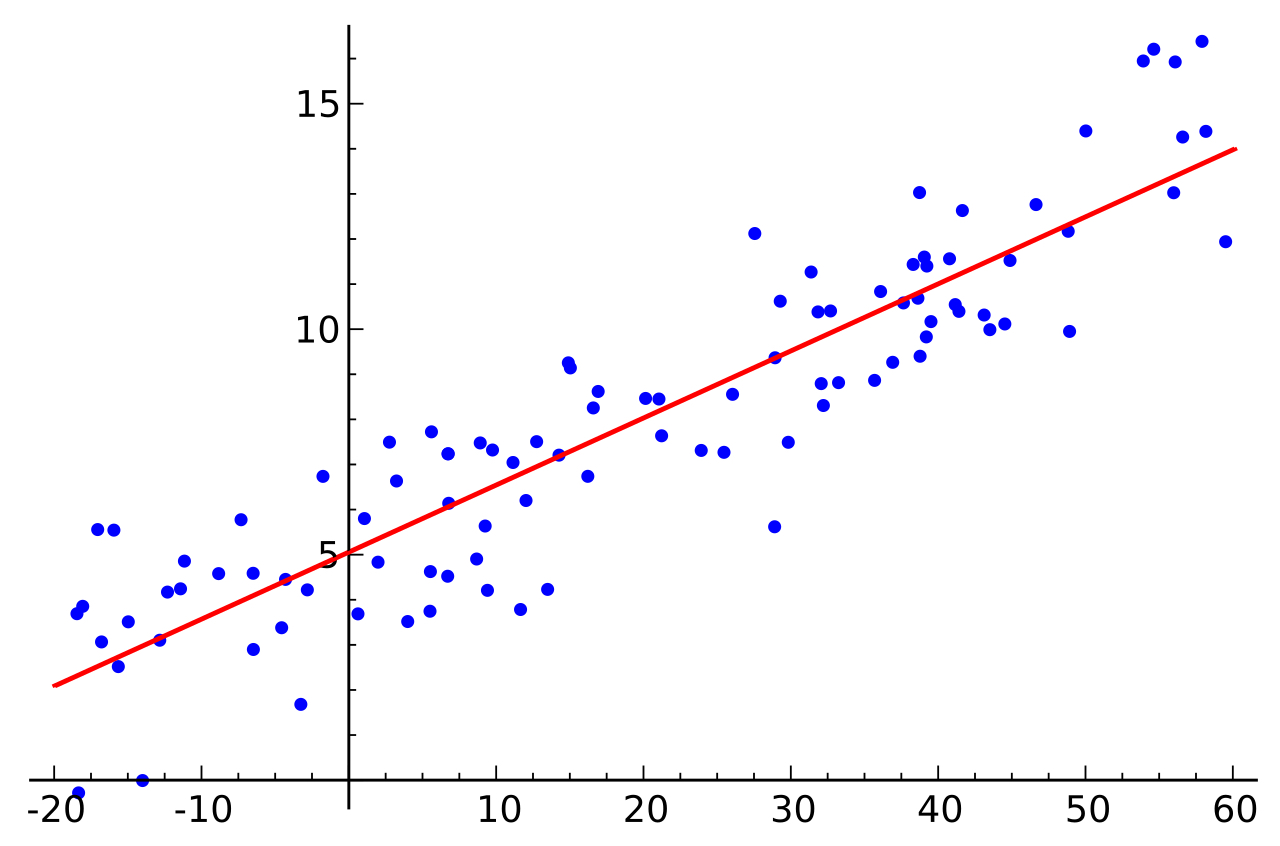
\includegraphics[width=8.5cm, height=3.5cm]{figures/1280px-Linear_regression.jpg}
			\caption{Imagen a la Izquierda}
			\label{Fig:ImagenALaIzquierda}
\end{wrapfigure}

Texto Texto Texto Texto Texto Texto Texto Texto Texto Texto Texto Texto Texto Texto Texto Texto Texto Texto Texto Texto
Texto Texto Texto Texto Texto Texto Texto Texto Texto Texto Texto Texto Texto Texto Texto Texto Texto Texto Texto Texto
Texto Texto Texto Texto Texto Texto Texto Texto Texto Texto Texto Texto Texto Texto

\begin{wrapfigure}[11]{r}[1pt]{8.5cm}
	    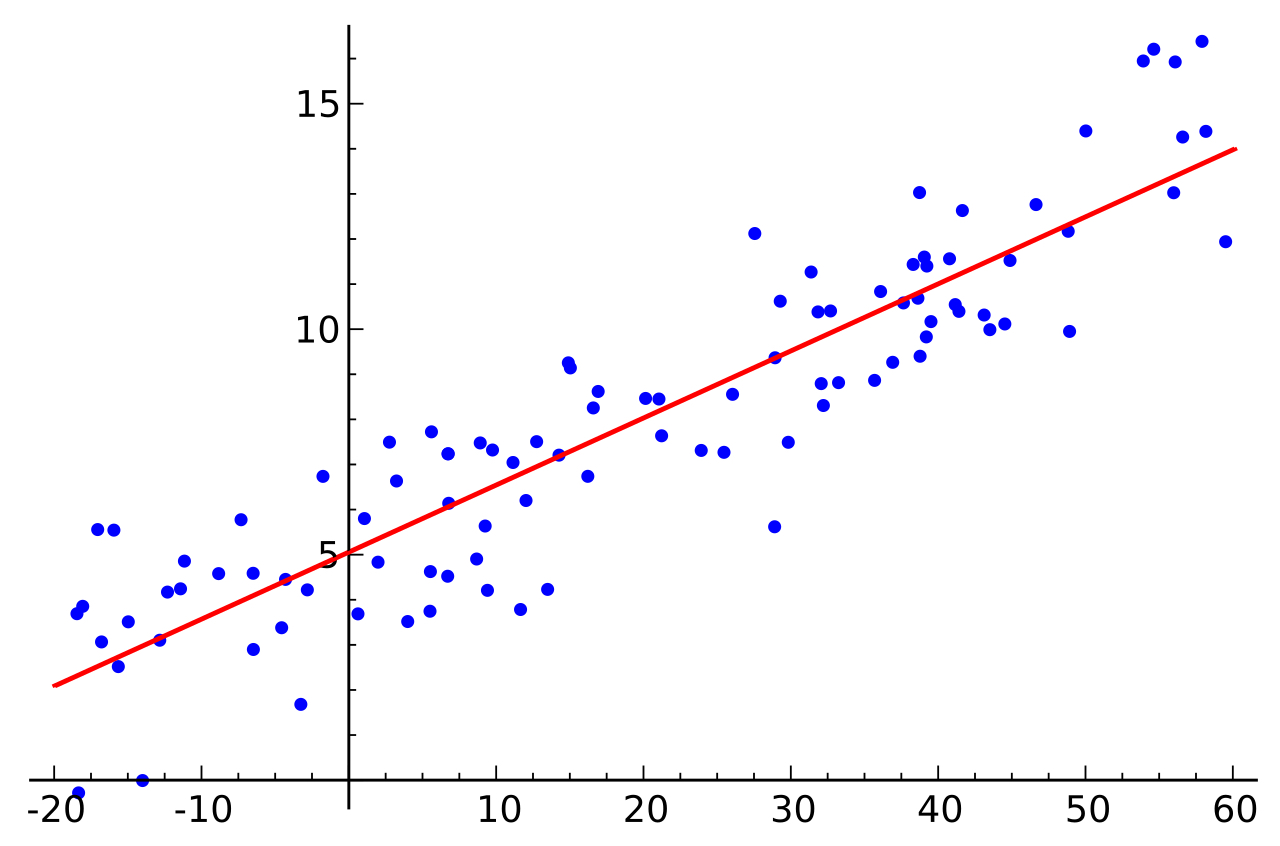
\includegraphics[width=8.5cm, height=3.5cm]{figures/1280px-Linear_regression.jpg}
			\caption{Imagen a la Derecha}
			\label{Fig:ImagenALaDerecha}
\end{wrapfigure}

Texto Texto Texto Texto Texto Texto Texto Texto Texto Texto Texto Texto Texto Texto Texto Texto Texto Texto Texto Texto
Texto Texto Texto Texto Texto Texto Texto Texto Texto Texto Texto Texto Texto Texto Texto Texto Texto Texto Texto Texto
Texto Texto Texto Texto Texto Texto Texto Texto Texto Texto Texto Texto Texto Texto 

\begin{figure}[ht]
	\centering
		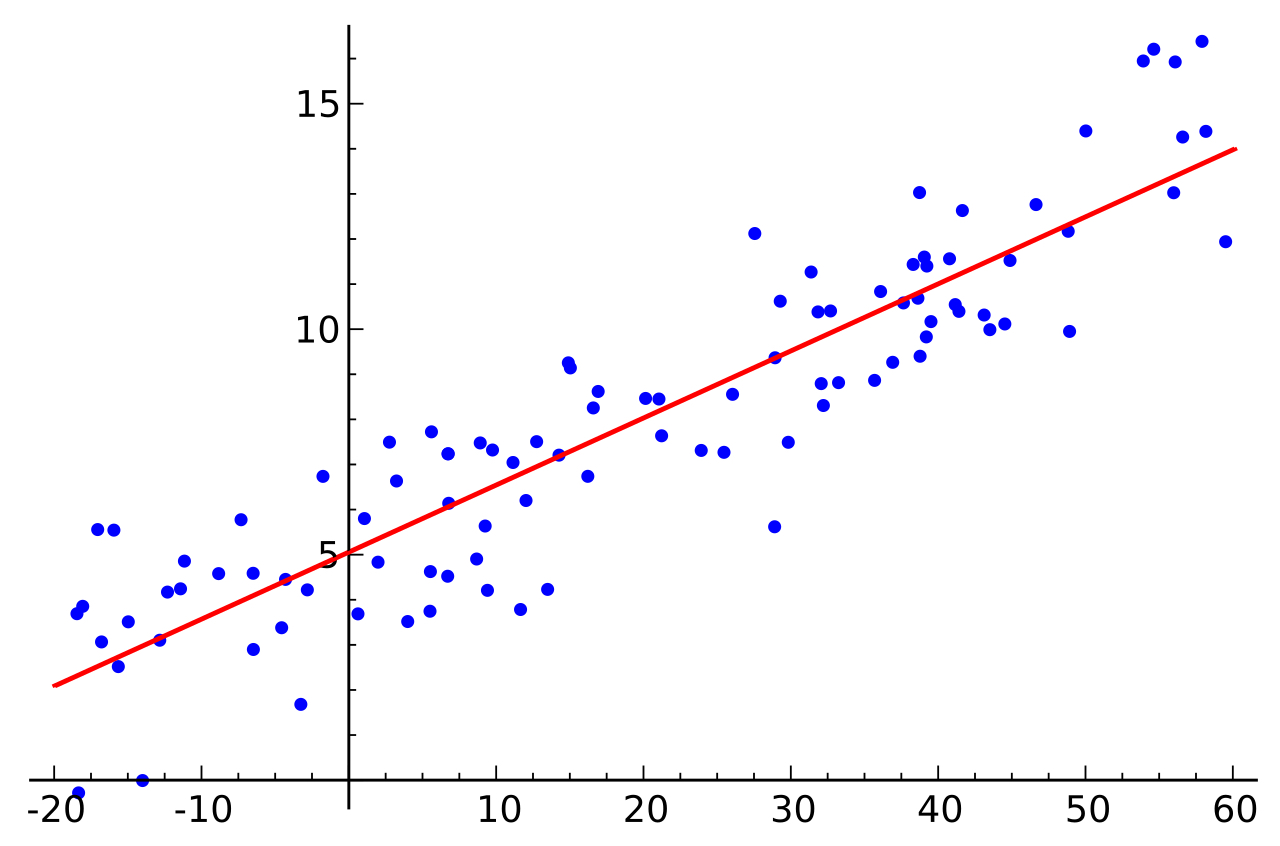
\includegraphics[width=5.5cm]{figures/1280px-Linear_regression.jpg}
	\caption{Imagen Centrada sin Texto}
	\label{Fig:CentradaSinTexto}
\end{figure}

\begin{figure}
   \begin{minipage}{.5\linewidth}
	    \centering
      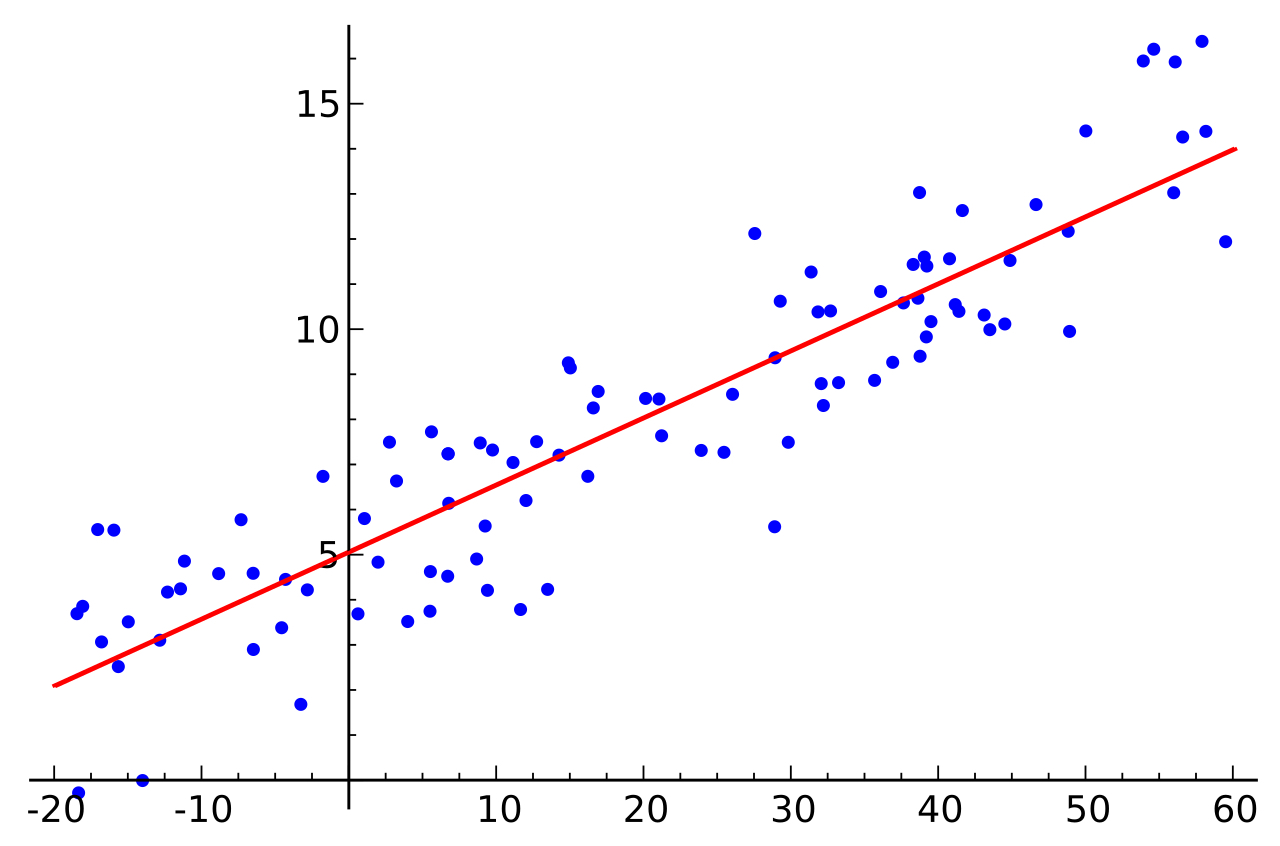
\includegraphics[width=7cm]{figures/1280px-Linear_regression.jpg}
      \caption{Imagen 1}
	 	  \label{Fig:Dos1}
   \end{minipage}%
   \begin{minipage}{.5\linewidth}
	    \centering
		  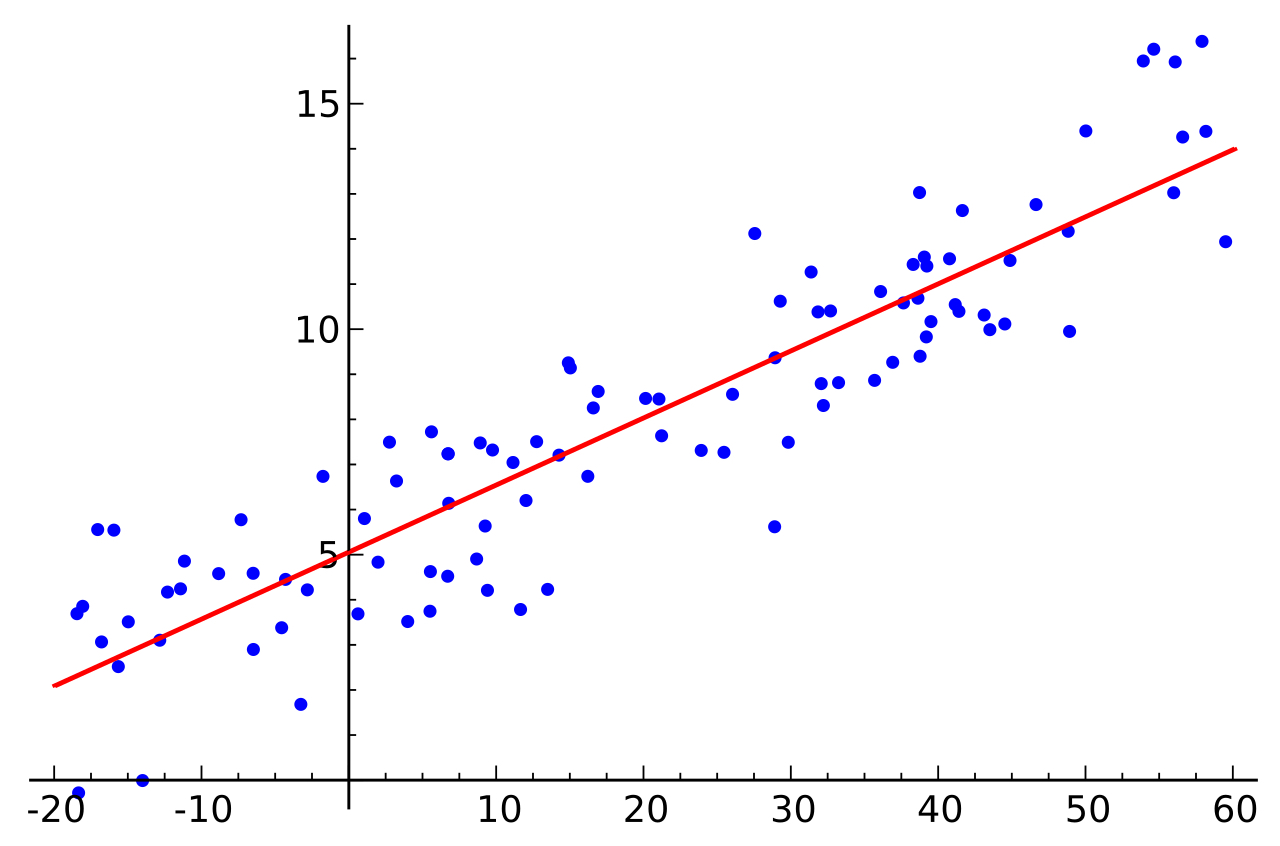
\includegraphics[width=4cm]{figures/1280px-Linear_regression.jpg}
      \caption{Imagen 2}
			\label{Fig:Dos2}
   \end{minipage}
\end{figure}

\newpage
\section{Apéndice B- Referencias Bibliográficas}
\label{Apx:Apendice_B}
%\include{Incluir Fichero Apéndice B}

Estas son algunas referencias bibliográficas, extraidas de \textbf{CiteSeer}:

Algunos libros que hacen referencia a Latex los encontramos en \cite{kreher05pseudocode}, \cite{ohl97emp}, \cite{smith-tools}, \cite{souza-mathematical}, \cite{braams-babel}, \cite{-basic}
